\documentclass[conference]{IEEEtran}

\usepackage{cite}
\usepackage[usenames,dvipsnames]{xcolor}
\usepackage{graphicx}
\usepackage{ifthen}
\usepackage{xspace}

\newboolean{showcomments}
\setboolean{showcomments}{true}

\ifthenelse{\boolean{showcomments}}
           { \newcommand{\mynote}[2]{%
               \fbox{\color{Red}\bfseries\sffamily\scriptsize#1}
               {\small\sffamily\color{BrickRed} #2}}
           }
           { \newcommand{\mynote}[2]{}}

\newcommand{\fabrice}[1]{\mynote{FK}{#1}}
\newcommand{\julien}[1]{\mynote{JS}{#1}}
\newcommand{\ludovic}[1]{\mynote{LLF}{#1}}
\newcommand{\soheib}[1]{\mynote{SB}{#1}}
\newcommand{\vincent}[1]{\mynote{VV}{#1}}

\newcommand{\painless}[0]{\texttt{Painless}\xspace}
\newcommand{\maple}[0]{\texttt{MapleCOMSPS}\xspace}
\newcommand{\pmcomsps}[0]{\texttt{P-MCOMSPS}\xspace}
\newcommand{\preduce}[0]{\texttt{P-MCOMSPS-STR}\xspace}

\begin{document}
\title{\texttt{P-MCOMSPS\{,-STR\}}: \painless-based Portfolios of \maple.}

\author{
   \IEEEauthorblockN{
      Vincent Vallade\IEEEauthorrefmark{1},
      Ludovic Le Frioux\IEEEauthorrefmark{2},
      Souheib Baarir\IEEEauthorrefmark{1}\IEEEauthorrefmark{3},
      Julien Sopena\IEEEauthorrefmark{1}\IEEEauthorrefmark{4},
      Fabrice Kordon\IEEEauthorrefmark{1}
   }
   \IEEEauthorblockA{
      \IEEEauthorrefmark{1}Sorbonne Universit\'e, LIP6, CNRS, UMR 7606, Paris,
      France
   }
   \IEEEauthorblockA{
      \IEEEauthorrefmark{2}LRDE, EPITA, Le Kremlin-Bic\^ectre, France
   }
   \IEEEauthorblockA{
      \IEEEauthorrefmark{3}Universit\'e Paris Nanterre, France
   }
   \IEEEauthorblockA{
      \IEEEauthorrefmark{4}INRIA, Delys Team, Paris, France
   }
}

\maketitle

\begin{abstract}
   This paper describes the two versions of the solver \pmcomsps submitted to
   the parallel track of the SAT Competition in 2020. They are concurrent
   portfolio solvers instantiated with PArallel INstantiabLE Sat Solver
   (\painless) framework and using \maple as core sequential solver.
\end{abstract}

\IEEEpeerreviewmaketitle

\section{Introduction}

\pmcomsps is a parallel SAT solvers built by instantiating components of the
\painless parallel framework~\cite{painless_17}. It is a Portfolio-based solver
implementing a diversification strategy, fine control of learnt clause
exchanges, and using \maple~\cite{maplecomsps_17} as a core sequential solver.
Morever \preduce is a version of \pmcomsps where learnt clause strengthening
has been integrated.

Section \ref{sec:painless} gives an overview on \painless framework. Section
\ref{sec:instance1} details the implementation of \pmcomsps using \painless and
\maple. Section \ref{sec:instance2} explains how learnt clause strengthening
has been incorporated in \pmcomsps to give the solver \preduce.

\section{Description of \painless}
\label{sec:painless}

\painless is a framework that aims at simplifying the implementation and
evaluation of parallel SAT solvers for many-core environments. Thanks to its
genericity and modularity, the components of \painless can be instantiated
independently to produce new complete solvers.

The main idea of the framework is to separate the technical components (e.g.,
those dedicated to the management of concurrent programming aspects) from those
implementing heuristics and optimizations embedded in a parallel SAT solver.
Hence, the developer of a (new) parallel solver concentrates his efforts on the
functional aspects, namely parallelization and sharing strategies, thus
delegating implementation issues (e.g., data concurrent access protection
mechanisms) to the framework.

Three main components arise when treating parallel SAT solvers:
\textit{sequential engines}, \textit{parallelization}, and \textit{sharing}.
These form the global architecture of \painless.

\subsection{Sequential Engines}

The core element that we consider in our framework is a sequential SAT solver.
This can be any CDCL state-of-the art solver. Technically, these engines are
operated through a generic interface providing basics of sequential solvers:
\textit{solve, interrupt, add clauses}, etc.

Thus, to instantiate \painless with a particular solver, one needs to implement
the interface according this engine.  

\subsection{Parallelization}

To built a parallel solver using the aforementioned engines, one needs to
define and implement a parallelization strategy. Portfolio and
Divide-and-Conquer are the basic known ones. Also, they can be arbitrary
composed to form new strategies.

In \painless, a strategy is represented by a tree-structure of arbitrary depth.
The internal nodes of the tree represent parallelization strategies, and leaves
are core engines. Technically, the internal nodes are implemented using
\texttt{WorkingStrategy} component and the leaves are instances of
\texttt{SequentialWorker} component. 

Hence, to develop its own parallelization strategy, the user should create one
or more strategies, and build  the required tree-structure.

\subsection{Sharing}

In parallel SAT solving, the exchange of learnt clauses warrants a particular
focus. Indeed, beside the theoretical aspects, a bad implementation of a good
sharing strategy may dramatically impact the solver's efficiency.

In \painless, solvers can export (import) clauses to (from) the others during
the resolution process. Technically, this is done by using lockfree
queues~\cite{lockfree-queues_96}. The sharing of these learnt clauses is
dedicated to particular components called \texttt{Sharers}. Each
\texttt{Sharer} in charge of sets of producers and consumers and its behaviour
reduces to a loop of sleeping and exchange phases. 

Hence, the only part requiring a particular implementation is the exchange
phase, that is user defined. 

\section{\pmcomsps}
\label{sec:instance1}

This section describes the overall behaviour of our competing instantiation
named \pmcomsps. Its architecture is highlighted in Fig.~\ref{fig:instance}.

\begin{figure}[t]
   \centering
   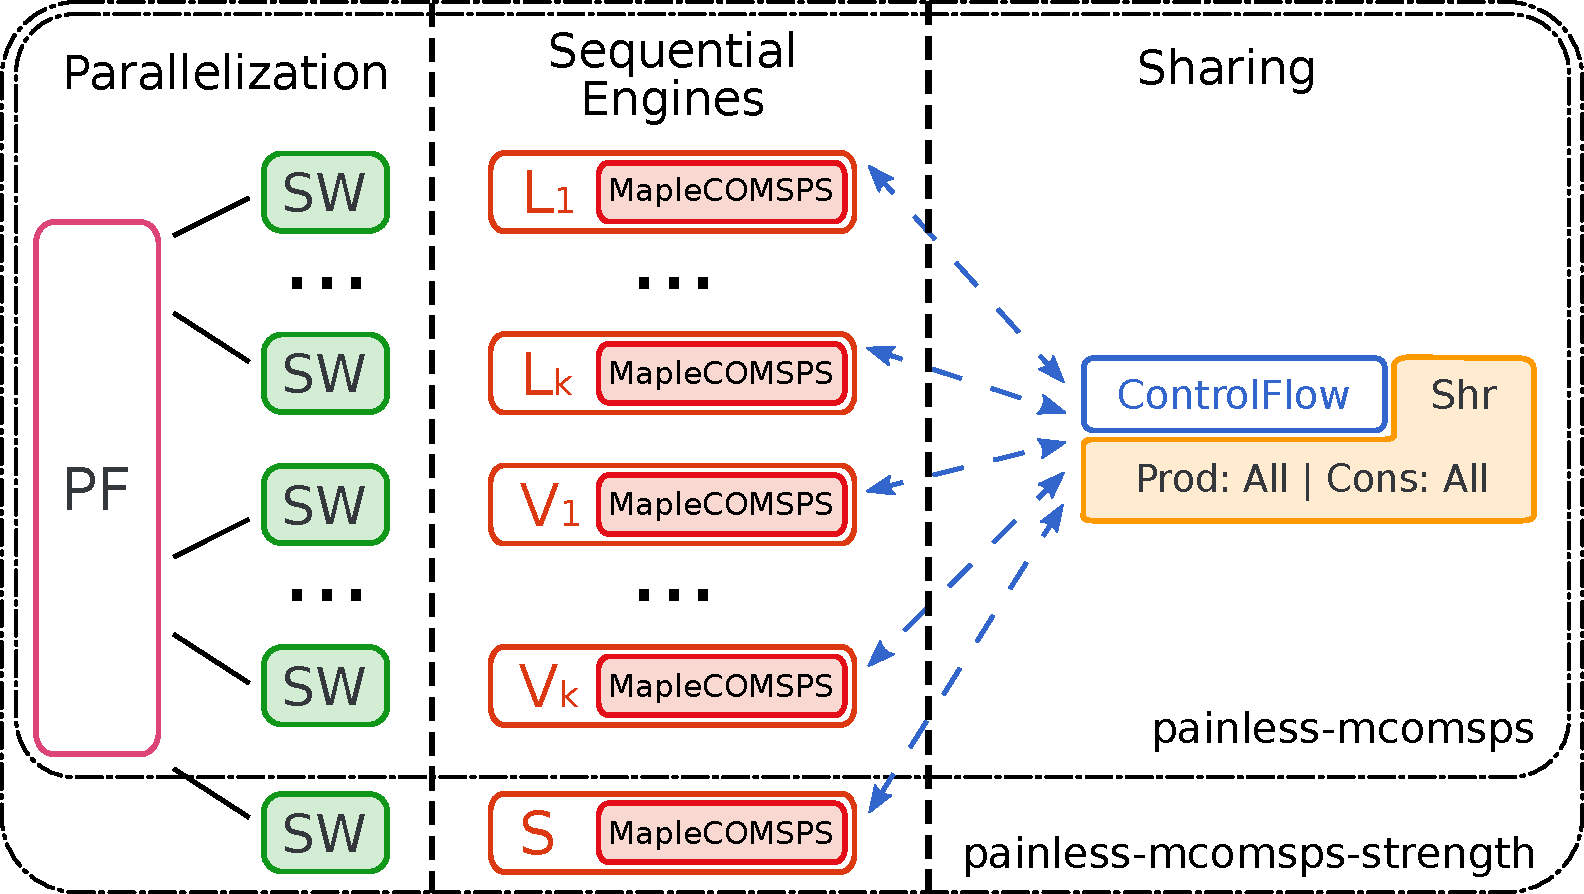
\includegraphics[scale=0.3]{figures/instance.pdf}
   \caption{Architecture of \pmcomsps.}
   \label{fig:instance}
\end{figure}

\ludovic{The figure should show normal + reduce mode.}

\subsection{Sequential Engines: \maple}

\maple is a sequential solver that finished second of the main track of the SAT
Competition 2017. It is based on \texttt{MiniSat}~\cite{minisat_03}, and uses
as decision heuristics the classical Variable State Independent Decaying Sum
(VSIDS)~\cite{vsids_01}, and newly defined Learning Rate Branching
(LRB)~\cite{lrb_16}. These heuristics are used in one-shot phases: first LRB,
then VSIDS. Moreover, it uses Gaussian Elimination (GE) at preprocessing time.

We adapt this solver for the parallel context as follows: (1) we parametrized
the solver to select either LRB, or VSIDS for all solving process (noted
respectively, \texttt{L} and \texttt{V}); (2) we added callbacks to export and
import clauses; (3) we added an option to use or not the GE preprocessing; (4)
we parametrized the solver to use as variable score comparator either $<$ or
$<=$ (noted respectively head: \texttt{H} and tail: \texttt{T}).

\subsection{Parallelization: Portfolio and Diversification}

\pmcomsps is a solver implementing a basic Portfolio strategy (\texttt{PF}),
where the underlying core engines are either \texttt{LH}, \texttt{LT},
\texttt{VH} or \texttt{VT} instances.

For each type of instances, we apply a sparse random diversification similar to
the one introduced in~\cite{hordesat_15}. That is for each group of $k$
solvers, the initial phase of a solver is randomly set according the following
settings: every variable gets a probability $1/2k$ to be set to false, $1/2k$
to true, and $1 - 1/k$ not to be set.

Moreover, only one of the solvers performs the GE preprocessing.

\subsection{Sharing: Controlling the Flow of Shared Clauses}

In \pmcomsps, the sharing strategy \texttt{ControlFlow} is inspired from the one
used by~\cite{hordesat_15,tcp_sharing_11}. We instantiate one \texttt{Sharer}
for which all solvers are producers. It gets clauses from this producer and
exports some of them to all others (the consumers).

The exchange strategy is  defined  as follows: each solver exports clauses
having a LBD value under a given threshold (2 at the beginning). Every 1.5
seconds, 1500 literals (the sum of the size of the shared clauses) are selected
by the \texttt{Sharer} and dispatched to consumers. The LBD threshold of the
concerned solver is increased (decrease) if an insufficient (a to big) number
of literals (respectively, less than 1125 and more than 1470) are dispatched.

\section{\preduce}
\label{sec:instance2}

This section describes the overall behaviour of our second competing
instantiation named \preduce. This solver is based on our solver \pmcomsps
described in Section~\ref{sec:instance1} and implements concurrent
strengthening~\cite{}.

\subsection{Sequential Engines: Strengthener}

The \textit{reducer} engine (\texttt{R}) of Fig.~\ref{fig:instance} implements
the algorithm introduced in~\cite{strength_13}.

We implemented the strengthening operation as a decorator of
\textit{SolverInterface}. This decorator is a \textit{SolverInterface} itself
that uses, by delegation, another \textit{SolverInterface} to apply the
strengthening, in the present case a \maple solver.

The reducer is part of the portfolio.

\subsection{Sharing: Online Strengthening}

The reducer engine is both a consumer and a producer of the sharer
(\texttt{Shr}). It receives clauses from the different cores, strengthened
them if possible, and exports them back after. The sharing mechanism will then
share this strengthen clauses.

Since, a strengthened clause subsumes the original one, it is likely that cores
will forget the original clause over time.

\section*{Acknowledgment}

We would like to thank Jia Hui Liang, Chanseok Oh, Vijay Ganesh, Krzysztof
Czarnecki, and Pascal Poupart, the authors of \maple.

\bibliographystyle{ieeetr}
\bibliography{biblio}

\end{document}
